\chapter{Détecteurs basés sur la scintillation}
\section{Introduction}
Quand un rayonnement ionisant interagit avec la matière, il peut ioniser ou exciter un grand
nombre de molécules qui, lorsqu'elles retournent dans l'état fondamental, peuvent créer un
centre de luminescence (émission de lumière par lors d'une recombinaison) dans le visible 
ou l'UV. On parle de \textit{radioluminescence, luminescence} ou \textit{scintillation}. Le 
nombre de photons émis $N_{h\nu}\propto E_{abs}$. La lumière émise est ensuite convertir en
impulsion électrique par un photomultiplicateur (PM) ou une photodiode.

\subsection{Luminescence}
Il existe trois types de luminescence
\begin{enumerate}
\item \textit{Fluorescence}. Durée de vie du centre de luminescence très court, l'émission de
lumière à lieu "immédiatement" après l'absorption.
\item \textit{Phosphorescence}. L'émission de lumière est retardée (état excité métastable).
\item \textit{Fluorescence retardé}. Un centre de phosphorescence est stimulé extérieurement et
devient un centre de fluorescence.
\end{enumerate}

Un bon scintillateur doit avoir plusieurs propriétés
\begin{itemize}
\item[$\bullet$] La conversion de l'énergie cinétique du rayonnement ionisant en photons détectables doit avoir une efficacité élevée.
\item[$\bullet$] $N_{h\nu} \propto E_{abs}$
\item[$\bullet$] Transparent à sa lumière de scintillation
\item[$\bullet$] Temps de vie du centre de luminescence nul ou très faible
\item[$\bullet$] Indice de réfraction proche du verre ($n\approx1.5$) pour éviter réflexion totale entre
le scintillateur et le PM
\item[$\bullet$] Chimiquement et mécaniquement stable
\item[$\bullet$] Peu cher
\end{itemize}\ 

Hélas, aucun matériau ne possède toutes ces propriétés, il faudra travailler par compromis (en plus
les dimensions du scintillateur dépendent du type de rayonnement (plus grande pour les $\gamma$)). Il
existe deux grande familles de scintillateur 
\begin{enumerate}
\item Organique : fluorescence d'origine moléculaire
\item Inorganique : fluorescence d'origine cristalline
\end{enumerate}
Il existe aussi des scintillateurs aux gaz rares avec une fluorescence d'origine atomique, mais ils
sont plus rarement utilisés.

\section{Scintillateurs organiques}%sl7
L'exemple du benzène est donné aux slides 7 à 9.


\subsection{Mécanismes de scintillation : Fluorescence}%sl10
Celle-ci se déroule en six étapes
\begin{enumerate}
\item Une particule ionisante traverse le scintillateur et produit des ionisations/excitations
\item Après absorption de l'énergie, la molécule passe dans un état électronique excité
\item Très rapidement, les états excités les plus élevés se désexcite sans émission de photons 
mettant la molécule dans l'état $S_1$
\item Transitions non-radiatives entre états vibrationnels vers l'état $S_{10}$
\item Désexcitation radiative vers un état $S_{0i}$ : fluorescence
\item Transition non radiative, état $S_{00}$.
\end{enumerate}




\subsection{Mécanismes de scintillation : Phosphorescence}%sl11
	\begin{wrapfigure}[10]{l}{5cm}
	\vspace{-5mm}
	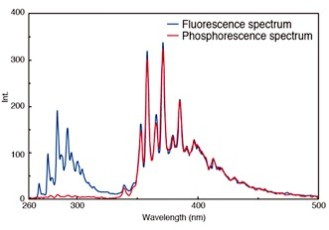
\includegraphics[scale=0.55]{ch10/image1}
	\captionof{figure}{ }
	\end{wrapfigure}
	
On retrouve le même processus pour les états triplets jusqu'à ce que les molécules soient dans
l'état $T_1$ (directement ou à partir de $S_1$). Les transitions $T_1\to S_0$ sont fortement 
interdites mais possibles : la durée de vie de l'état $T_1$ et longue et l'émission est différée,
il s'agit de la phosphorescence. Comme les niveaux $T < $ niveaux $S$, la longueur d'onde de la
phosphorescence est plus grande que celle de la fluorescence.\\



\subsection{Mécanismes de scintillation: Fluorescence retardée}%sl13
Dans l'état métastable $T_{10}$, les molécules peuvent être excitées vers l'état $S_{10}$ par 
un stimulus extérieur contrôlé pour faire de la fluorescence retardée.


\subsection{Propriétés des scintillateurs organiques}%sl14
L'énergie de transition $S_{10}\to S_{0i}$ est plus faible que l'énergie de transition
$S_{00}\to S_{1i}$, les spectres d'émission et d'absorption ne se superposent que de peu
(décalage de \textsc{Stokes}). Un scintillateur est alors quasi transparent à sa propre
lumière de luminescence.


\subsubsection{Réponse lumineuse d'un scintillateur organique}%sl16
	\begin{wrapfigure}[5]{r}{3cm}
	\vspace{-5mm}
	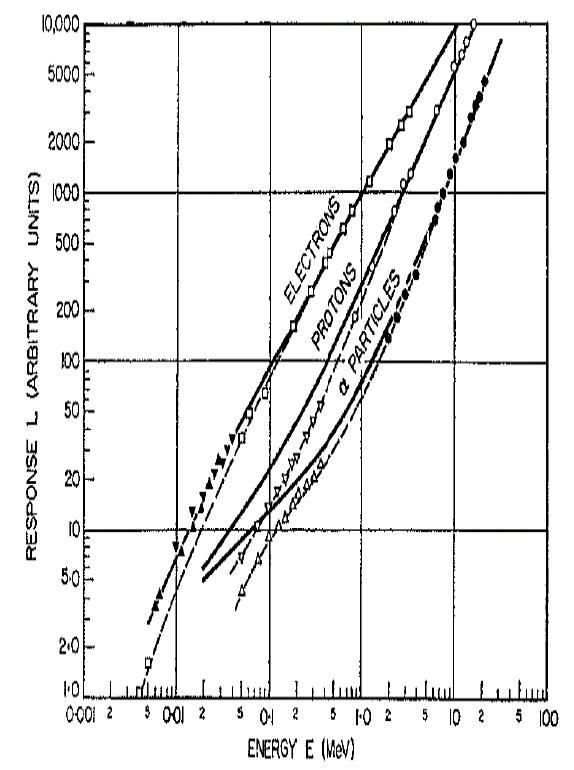
\includegraphics[scale=0.2]{ch10/image2}
	\captionof{figure}{ }
	\end{wrapfigure}
Seule une petite partie de l'énergie cinétique perdue par le rayonnement incident est 
convertie en énergie de fluorescence. Le reste est dissipé de façon non-radiative, 
principalement en chaleur. La \textbf{réponse lumineuse du scintillateur} $L$ est l'énergie
émise par fluorescence
\begin{equation}
L=E_{h\nu}=\langle N_{h\nu}\rangle \langle h\nu\rangle
\end{equation}
avec $\langle N_{h\nu}\rangle$ ne nombre moyen de photons émis et $\langle h\nu\rangle$ leur 
énergie moyenne. L'efficacité intrinsèque du scintillateur se définit comme
\begin{equation}
S=\frac{L}{E_{abs}}
\end{equation}
où $S$ est généralement faible. L'énergie moyenne perdue $W$ pour chaque photon émis vaut alors
\begin{equation}
W=\frac{E_{abs}}{\langle N_{h\nu}\rangle}=\frac{\langle h\nu\rangle}{S}
\end{equation}
Avec $\langle h\nu\rangle \approx 2-3$ eV et $W\approx100$ eV. Notons que $S$ et $W$ dépendent
fortement du type de rayonnement incident et parfois de son énergie.\\

Discutons-en, sachant que $L = SE_{abs}$
\begin{itemize}
\item[$\bullet$] Pour des particules à faible densité d'ionisation, la distance entre deux collisions
successives est grande comparée à la distance entre deux molécules voisine. L'interaction entre deux
sites luminescent est faible et $S$ et indépendant de $E_{abs}$ (réponse linéaire).
\item[$\bullet$] Les particules lourdes (proton, $\alpha$, \dots) présentent une densité d'ionisation
plus grande. Les sites sont plus proches et peuvent interagir\footnote{Il n'y a pas encore de 
théorie clair sur comment ils interagissent.} ce qui cause une diminution de l'émission lumineuse, 
$S$ est donc dépendant de $E_{abs}$.
\end{itemize}


\subsubsection{Réponse lumineuse différentielle d'un scintillateur}%sl20
	\begin{wrapfigure}[10]{r}{6.2cm}
	\vspace{-15mm}
	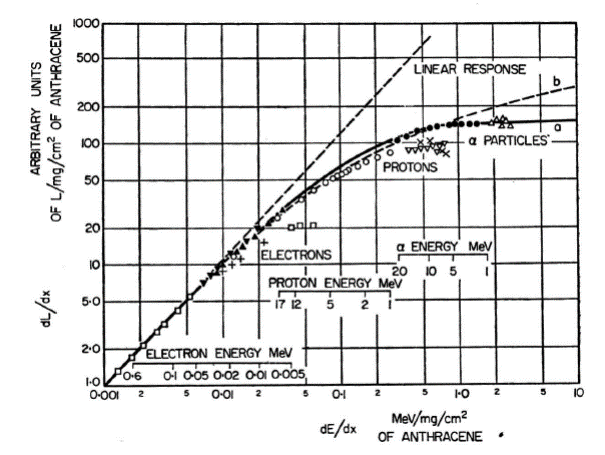
\includegraphics[scale=0.4]{ch10/image3}
	\captionof{figure}{ }
	\end{wrapfigure}
La réponse lumineuse différentielle du scintillateur $dL/dx$ est l'énergie fluorescente $dL$ émise
par unité de distance parcourue par la particule ionisante
\begin{equation}
\frac{dL}{dx}=S\frac{dE_{abs}}{dx}
\end{equation}
où $dE_{abs}/dx$ est le pouvoir d'arrêt. Pour un faible pouvoir d'arrêt, la densité d'ionisation 
est faible de $S$ est constant. De façon plus générale, la réponse lumineuse différentielle suit
la loi de \textsc{Birks}. \\

Supposons que la densité d'ionisation et d'excitation est proportionnelle au pouvoir d'arrêt. On 
introduit alors le \textit{paramètre de quenching} $k$ qui est le facteur de proportionnalité entre 
la fraction des centres de luminescence qui "disparaissent" et la densité d'ionisation. Plus $k$ 
augmente, plus c'est embêtant. Sans quenching, on trouve
\begin{equation}
\frac{dL}{dx}=S_n\frac{dE_{abs}}{dx}
\end{equation}
où $S_n$ est l'efficacité normale du scintillateur, indépendante de l'énergie. Si on tient compte
du quenching, on obtient la formule de \textsc{Birks}
\begin{equation}
\frac{dL}{dx}=\frac{S_n(dE_{abs}/dx)}{1+kB(dE_{abs}/dx)}
\end{equation}
où l'on retrouve la formule d'avant pour $k=0$ ce qui se retrouve également lorsque $dE_{abs}/dx$ 
est petit. Si par contre il est grand
\begin{equation}
\frac{dL}{dx}=\frac{S_n}{kB}
\end{equation}
où $kB$ est un paramètre ajustable permettant de faire correspondre la pratique à l'expérience.

\newpage
\subsubsection{Réponse temporelle d’un scintillateur organique }%sl24
La variation de l'intensité lumineuse en fonction du temps dépend du temps de formation $\tau_1$ des
centres de luminescence et de la durée de vie $\tau$ de ces centres. L'expression de 
\textsc{Hyman} nous donne cette variation 
\begin{equation}
I=I_0\left(e^{-t/\tau}-e^{-t/\tau_1}\right)
\end{equation}
Le grand avantage des scintillateurs organiques est la réponse extrêmement rapide qui permet souvent
d'ignorer le temps de formation du centre de luminescence. Par contre à température ambiante, on 
ne peut pas négliger la fluorescence retardée due à la stimulation thermique. On va en tenir compte
en ajoutant une exponentielle décroissante. Posons $\tau_r$, la durée de vie des centres retardés
\begin{equation}
I=Ae^{-t/\tau}+Be^{-t/\tau_r}
\end{equation}
où le premier terme est la composante rapide de la scintillation et la seconde la lente.  Notons que
$\tau_r$ dépend du type de particule incidente et donc du quenching et finalement de la densité 
d'ionisation.







\subsubsection{Types de scintillateurs organiques}
Une brève description est donnée aux slides
27 et 28.

\section{Scintillateurs inorganiques}%sl30

\subsection{Description des scintillateurs inorganiques et mécanismes de scintillations}%sl31
Le mécanisme de scintillation dépend de la structure en bande du cristal. Si le cristal est
pur, le gap est généralement trop important (6-7 eV) et ce n'est pas dans le visible (3-4 eV). Pour
se faire, on va ajouter des impuretés (\textit{activateurs}). Ceux-ci vont ajouter des 
niveau dans la bande interdite afin que les recombinaisons produisent des photons de plus faibles
énergies, dans le visible. De plus, au énergie plus faible la probabilité de transition est plus
élevée et on peut plus faire passer des électrons de la bande de valence à celle de conduction ce 
qui est favorable.\\

Après excitation, le trou migre vers un site d'activation et se fait piégé : il crée alors un
centre de recombinaison. Pour l'électron, après l'excitation, il migre puis plusieurs processus
sont possibles
\begin{enumerate}
\item Migre vers un centre de luminescence et il y a émission d'un photon
\item Migre vers un site d'impureté ou la transition vers le fondamentale est interdite, il se 
retrouve piégé.  Avec de l'énergie thermique il peut remonter vers la bande de conduction puis
se faire capturer par un centre de luminescence : fluorescence retardée
\item Capturé par un centre de quenching (coupure, tout ce qui limite un phénomène), c'est à dire 
un centre de désexcitation non-radiatif. C'est un mécanisme de perte, le rendement diminue.
\item L'électron et le trou forment un état lié, l'exciton, qui migre jusqu'à un centre d'impureté
où il y ara émission d'un photon.
\end{enumerate}

\subsection{Propriétés des scintillateurs inorganiques}%sl35
Le temps de vie des centres de recombinaisons est 2 à 3 ordres plus lent que les scintillateurs
organiques. Ceci à une conséquence sur la luminescence via les activateurs : l'énergie libérée
durant la luminescence est inférieure à celle nécessaire pour la création d'une paire. Les 
spectres d'émission/absorption ne se superposent pas et il est donc transparent à sa propre 
lumière. Il faut bien sur éviter le recouvrement des deux spectres sans quoi on aurait de 
l'auto-absorption ce n'est pas génial.\\

Ils ont généralement un $Z$ élevé et donc un bon pouvoir d'arrêt, particulièrement adapté à 
la spectro $\gamma$ avec une efficacité de luminescence élevé. Ils absorbent par contre 
énormément d'humidité et ils faut les protéger. Les particules lourdes ont une probabilité de
quenching plus élevé et la présence de non-linéarité ce qui fait que ce détecteur n'est pas
adapté pour de telles particules. Il y a également de fortes variation de l'efficacité de 
luminescence en fonction de la température.
\begin{itemize}
\item[$\bullet$] A faible températures, les paires sont piégés dans des pièges peu profonds.
\item[$\bullet$] Quand $T$ augmente, les paires sont libérées et peuvent atteindre les centres
de luminescences.
\item[$\bullet$] Lorsque $T$ augmente encore, les interactions entre les molécules augmente à
cause du quenching thermique (tout ce qui est pas bon). Au lieu d'avoir des recombinaisons, 
les électrons vont sauter d'un site à l'autre.
\end{itemize}

\subsubsection{Spectrométrie d'électron à l'aide d'un scintillateur}
La fonction de réponse présente un pic d'absorption total et une queue aux basses énergies à 
cause des électrons rétrodiffusés. Cette rétrodiffusion dépend fortement du $Z$ : la probabilité
de rétrodiffusion augmente avec $Z$. En plus, augmenter $Z$ augmente le Bremsstrahlung et plus
d'énergie s'échappe du détecteur. On favorisera ainsi les matériau à petit $Z$, soit des 
scintillateurs organiques, pour la détection d'électron (à l'opposé de la spectro $\gamma$).


\subsubsection{Types de scintillateurs inorganiques}
Grossièrement classés en trois groupes
\begin{enumerate}
\item Dopés par des impuretés
\item Non dopés mais auto-activés
\item Purs
\end{enumerate}


\subsection{NaI(Tl)}%sl44
Il s'agit d'un cristal d'iodure de sodium dopé avec du thallium. Proposé comme détecteur en 
\textit{1948} par \textsc{Hofstadter}, il possède un rendement élevé. Il s'agit du scintillateur
le plus utilisé mais qui est fortement hygroscopique.\\

	\begin{wrapfigure}[9]{l}{6.5cm}
	\vspace{-5mm}
	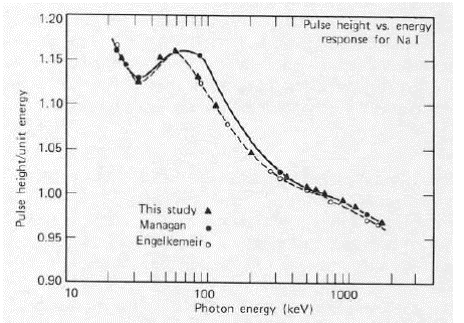
\includegraphics[scale=0.55]{ch10/image4}
	\captionof{figure}{ }
	\end{wrapfigure}
Le NaI pur possède un gap de 6 eV. Par contre, le NaI(Tl) a lui un gap de 3 eV pour une concentration
de 0.1\% en Tl. Son indice de réfraction estu un peu trop elevé (1.85) et son efficacité 
intrinsèque vaut $S\approx11\%$. Le facteur de \textsc{Fano} vaut 1 et $W=26$ ce qui est élevé : 
le principal défaut du NaI(Tl) est sa résolution élevée. Son efficacité intrinsèque de détection
devrait être linéaire mais l'écart peut atteindre 15\% : jusqu'à présent, on ne sait pas encore
pourquoi.

\newpage
\section{Photomultiplicateur}%sl53
Le but d'un PM est de convertir l'énergie d'un rayonnement visible (ou proche) en une énergie
électrique via des phénomène de photoémission et ensuite d'amplification grâce au processus
d'émission secondaire. Il s'agit d'une enceinte de verre dans laquelle règle le vide. Quand un
photon pénètre dans le PM, il frappe la photocathode semi-transparante. L'interaction du photon 
avec les atomes de la photocathode rend possible l'éjection d'un électron. Les photoélectrons 
sont ensuite accéléré par un champ électrique hors de la première dynode puis vont vers une 
seconde, etc jusqu'à être collecté par l'anode et former le signal. 



\subsection{Photocathode}%sl54
Si celle-ci est mince, les électrons peuvent sortir par la surface opposée à la surface d'entrée
des photons incidents. L'histoire se raconte en cinq parties
\begin{enumerate}
\item Un doit traverser la fenêtre d'entrée (épaisseur $e$) du PM : probabilité $T(\lambda,e)$. Il y
a en effet toujours un élément protecteur.
\item Il peut être réfléchi, absorbé ou transmis. Soit $\rho,\alpha$ et $\tau$, les probabilités
de ces trois processus
\begin{equation}
\rho(\lambda)+\alpha(\lambda)+\tau(\lambda)=1
\end{equation}
Pour pénétrer dans la photocathode, le matériau qui la constitue doit avoir un faible coefficient
de réflexion.
\item Le photon rentré doit être absorbé. Soit $\mu(\lambda)$ la probabilité d'absorption par 
unité de longueur. La probabilité que le photon soit absorbé à une profondeur $x$ dans l'intervalle
d$x$ est donné par
\begin{equation}
p_{abs}(x)dx=e^{-\mu(\lambda) x}\mu(\lambda) dx
\end{equation}
Si l'incidence est normale sur un matériau d'épaisseur $d$, on trouve
\begin{equation}
\alpha(\lambda,d)=[1-\rho(\lambda)]\left(1-e^{-\mu(\lambda)d}\right)
\end{equation}
\item Le matériau doit avoir une grande profondeur d'échappement (profondeur d'origine de 
l'électron telle qu'il peut atteindre la surface avec suffisamment d'énergie) sans quoi pas de 
signal.
\item L'électron doit s'échapper de la photocathode, son énergie doit donc être supérieur au 
travail d'extraction $\Phi$ de celle-ci.
\end{enumerate}\ \\

On peut définir le rendement quantique photoélectrique
\begin{equation}
\eta_{ph}(\lambda)=\frac{\mbox{nombre d'e$^-$ \'emis par la photocathode}}{\mbox{nombre de photons absorb\'es par la photocathode}}
\end{equation}
Mais aussi le rendement quantique spectral
\begin{equation}
\eta(\lambda)=\frac{\mbox{nombre d'e$^-$ \'emis par la photocathode}}{\mbox{nombre de photons p\'en\'etrant dans le PM}}
\end{equation}
Grâce à ces définitions, on a donc
\begin{equation}
\eta(\lambda)=T(\lambda,e)\alpha(\lambda,d)\eta_{ph}(\lambda)
\end{equation}
On défini aussi le rendement quantique effectif d'un photomultiplicateur qui reçoit une lumière dont
le spectre est $I(\lambda)$
\begin{equation}
\eta_{eff}=\int_0^\infty I(\lambda)\eta(\lambda)d\lambda
\end{equation}
Voir slides 58 - 59 pour le choix du matériau pour la photocathode.

\subsection{Bruit, gain de la photocathode et dynode}
A cause de l'agitation thermique, la photocathode émet spontanément des électrons. Ce nombre moyen
d'électrons émis par unité de temps et de surface est donné par la loi de \textsc{Richardson}
\begin{equation}
\eta_e=AT^2\exp{(-e\Phi/kT)}
\end{equation}
où $A$ est une constante. Comme $\Phi$ est plus petit pour un SC qu'un métal, $\eta_e$ est 
plus grand pour un SC. Si la température diminue $\eta_e$ fait de même mais d'autre sources de
bruit existent.\\

Après la photocathode, on arrive à la ne dynode. L'énergie de l'électron est transférée aux électrons
de la dynode et certains électrons sont arrachés. Chaque dynode apporte un gain défini par le 
rendement d'émission secondaire $\delta$ (forcément supérieur à 1 sinon pas de multiplication). Entre
les dynodes se trouve un champ électrique pour accélérer et guider les électrons. Le gain 
typique d'un PM vaut $M=\delta^n$ avec $n\approx10$ pour obtenir $M=10^7$. \\

	\begin{wrapfigure}[6]{l}{5.5cm}
	\vspace{-5mm}
	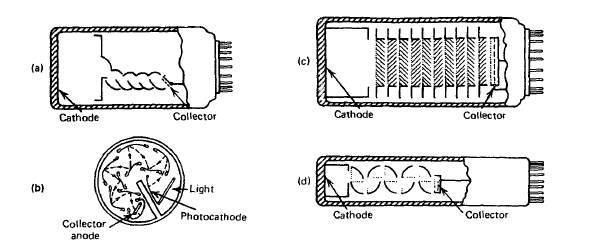
\includegraphics[scale=0.35]{ch10/image5}
	\captionof{figure}{ }
	\end{wrapfigure}
Si chaque électron qui frappe une dynode éjecte 4 électron, le gain d'un PM à 12 étage vaut
$4^12 \approx 1.7\times 10^7$. Un seul photoélectron produit donc 17 millions d'électrons qui arrivent
quasi tout en même temps à l'anode. L'impulsion de courant à l'anode vaut à peu près 0.5 mA.\\


\subsection{Résolution d'un détecteur à scintillation}%sl66

	\begin{wrapfigure}[12]{l}{4.5cm}
	\vspace{-5mm}
	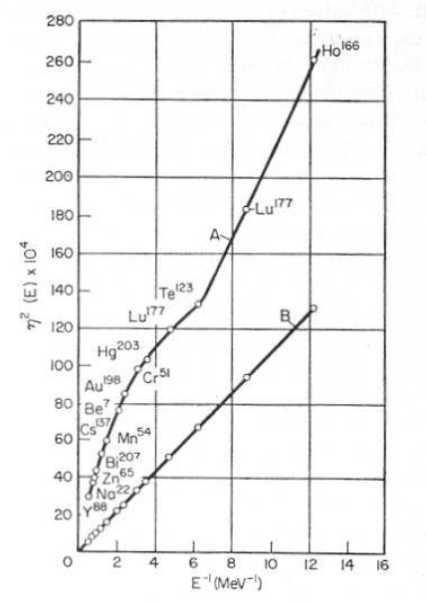
\includegraphics[scale=0.35]{ch10/image6}
	\captionof{figure}{On voit l'écart par rapport à la loi en $1/E_{abs}$}
	\end{wrapfigure}

Le détecteur à scintillation est donc la combinaison d'un scintillateur et d'un PM. Soit $C$, la
probabilité qu'un électron atteigne la première dynode, $N_0$ le nombre de photons collectés à 
l'anode et $N_{ph}$ le nombre de photons émis dans le scintillateur
\begin{equation}
N_0=MC\eta N_{ph}
\end{equation}
On voit donc que $N_0 \propto E_{abs}$. Comme il ne s'agit que de variables aléatoires, on peut 
calculer la variance. En posant $v[X]$ la variance relative de la variable aléatoire $X$
\begin{equation}
v[X]=\frac{\sigma^2(X)}{\langle X\rangle^2}
\end{equation}
On trouve, pour $v[N_0]$\footnote{On peut refaire le calcul théorique si on veut.}
\begin{eqnarray}
v[N_0]&=&v[N_{ph}]+\frac{1}{\langle N_{ph}\rangle}v[\eta]+\frac{1}{\langle N_{ph}\rangle\langle \eta\rangle}v[C]+\frac{1}{\langle N_{ph}\rangle\langle\eta\rangle\langle C\rangle}v[M]\\
&=&\left( v[N_{ph}]-\frac{1}{\langle N_{ph}\rangle}\right)+\frac{1}{\langle N_{ph}\rangle}\left( v[\eta]-\frac{1-\langle\eta\rangle}{\langle\eta\rangle}\right)\\
&&+\frac{1}{\langle N_{ph}\rangle \langle \eta\rangle}\left( v[C]-\frac{1-\langle C\rangle}{\langle C\rangle}\right)+\frac{1}{\langle N_{ph}\rangle\langle \eta\rangle\langle C\rangle}(1+v[M])
\end{eqnarray}
Si $N_{ph}$ est une variable de poisson et $C,\eta$ des binomiales
\begin{equation}
v[N_0]=\frac{1}{\langle N_{ph}\rangle\langle \eta\rangle\langle C\rangle}(1+v[M])\propto\frac{1}{E_{abs}}
\end{equation}
On obtient cette première loi théorique qui est en réalité totalement fausse à cause des effets
non-linéaires.


\section{Spectrométrie $\gamma$ avec un NaI(Tl)}
Premièrement, insistons sur le fait que \textbf{la taille du détecteur est un paramètre crucial} ! 
La taille doit être comparée au libre parcours moyen des $\gamma$ secondares dus aux interaction
du $\gamma$ incident qui est de 3-5cm dans le NaI. On considèrera pour la suite un détecteur de
longueur 7.62cm.


\subsection{$\gamma$ d'1 MeV}
Le processus dominant es la diffusion \textsc{Compton} : on suppose qu'ils en subissent tous 
exactement une avant de s'échapper sur le graphique du milieu. On suppose qu'ils en subissent
$n$ avant de s'échapper sur le graphique de droite.

\begin{center}
	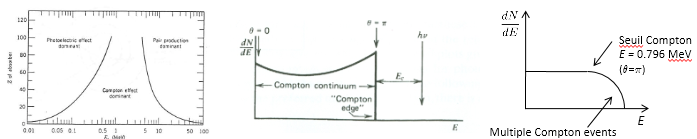
\includegraphics[scale=0.75]{ch10/image7}
	\captionof{figure}{ }
\end{center}


	\begin{wrapfigure}[6]{l}{7cm}
	\vspace{-5mm}
	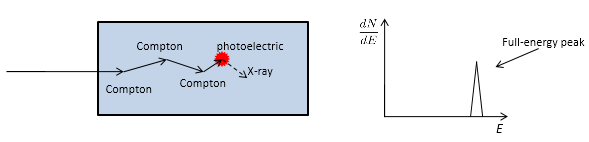
\includegraphics[scale=0.4]{ch10/image8}
	\captionof{figure}{ }
	\end{wrapfigure}
Après $n$ diffusion \textsc{Compton}, l'énergie diminue jusque $E_n$ et l'effet photoélectrique
devient dominant. Supposons qu'il se produit toujours et que $E_n-B_k$ est absorbé. Comme il 
se produit profondément dans le détecteur, les $RX$ ou les électrons d'\textsc{Auger} ne peuvent
pas s'échapper et une énergie $B_k$ est à nouveau déposé. Un pic d'absorption totale est observé.



\begin{center}
	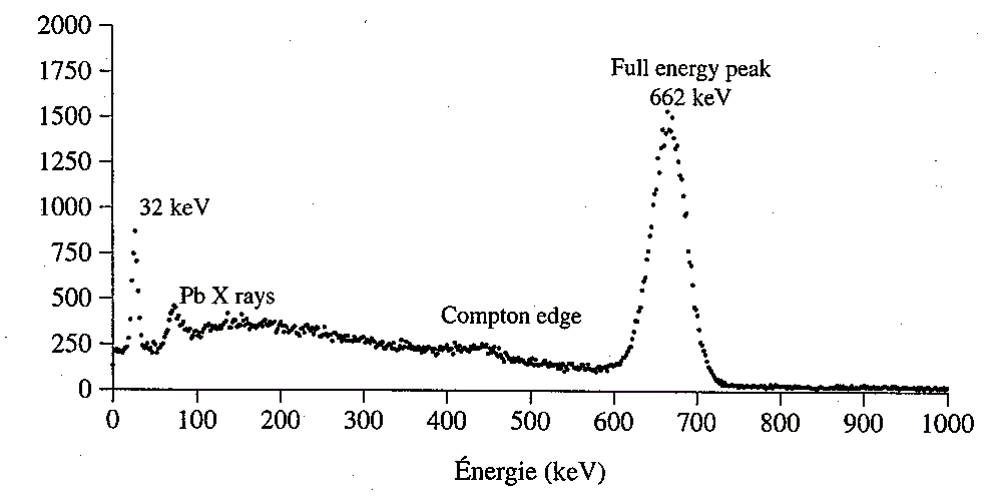
\includegraphics[scale=0.4]{ch10/image9}
	\captionof{figure}{En pratique, le $\gamma$ diffusé peut s'échapper après quelques diffusion
	\textsc{Compton} ou être absorbé. Ici l'exemple du $^{137}$Cs.}
\end{center}


\subsection{$\gamma$ de 100 keV}
	\begin{wrapfigure}[4]{l}{6.5cm}
	\vspace{-5mm}
	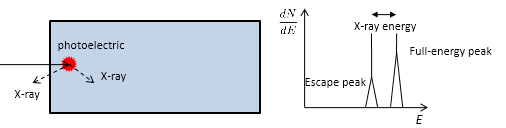
\includegraphics[scale=0.5]{ch10/image10}
	\captionof{figure}{ }
	\end{wrapfigure}
Le processus dominant est l'absorption photoélectrique. Le rayon $X$ d'énergie $E=B_k-B_L$ peut 
s'échapper (l'absorption se produit près de la surface d'entrée).\\


\subsection{$\gamma$ de 10 MeV}
	\begin{wrapfigure}[6]{l}{6.5cm}
	\vspace{-7mm}
	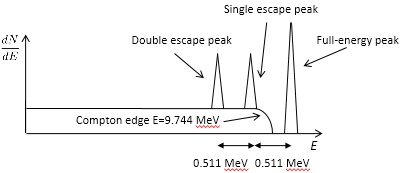
\includegraphics[scale=0.6]{ch10/image11}
	\captionof{figure}{ }
	\end{wrapfigure}
Le processus dominant est la diffusion \textsc{Compton} ou la création de paire. S'il y a création
 de paire, l'énergie déposée est de $E_0-2m_ec^2$ (avec $m_ec^2=0.511$ MeV). Les deux $\gamma$ 
 peuvent s'échapper, ou 1 peut s'échapper ou les deux peuvent être détecté (\textsc{Compton} ou
 photoélectrique).\\
 

\subsection{Complications de la réponse}
Les rayonnements secondaires créés à proximité de la source causent deux complications
\begin{enumerate}
\item Rayonnement d'annihilation. Si la source émet des positrons, un pic additionnel à 
511 keV sera mesurer à cause de l'annihilation dans la source ou le voisinage. Tout émetteur de
positron va émettre ce $\gamma$.
\item Bremsstrahlung. Les émetteurs de $\gamma$ sont généralement aussi émetteurs de $\beta$. Il 
faut stopper ces $\beta$ pour éviter qu'ils ne déposent leur énergie. Pour ça, on entoure la source
par un matériau placé avant le détecteur. Pour éviter le Bremsstrahlung, l'abosrbant des $\beta$
doit avoir un petit $Z$.
\end{enumerate}


L'effet de matériaux aux alentours (blindage) complique également pour trois raisons
\begin{enumerate}
\item Un rayon $X$ provenant du blindage peut être détecté
\item Si un photon traverse le détecteur il peut se faire rétrodiffusé et revenir au détecteur avec une énergie de 255 keV.
\item Il peut interagir avec le blindage et émettre le fameux pic à 511 keV d'annihilation causés par les positrons.
\end{enumerate}















